\section{Appendix: Additional Table and Graphs}\label{appendix:more_tables}
This section contains a table on precision, recall and F1 measures of the three different types of thresholding methods in selecting the non-zero entries of the spectral density matrices of VMA and VAR models of different dimension using different  sample sizes. The simulation settings are described in Section \ref{sec:simulation}. 

We also present enlarged images of the adjacency matrices of coherence networks obtained using adaptive lasso thresholding and shrinkage methods on the real data analysis in Section \ref{sec:realdata}. These images contain names of brain regions so that interesting strong connectivity patterns between regions can be identified easily.

\begin{sidewaystable}
\tiny
\centering
\def~{\hphantom{0}}
\begin{tabular}{l@{\hskip 0.4in} ccc ccc ccc}
& \multicolumn{3}{c}{Hard Thresholding}  & \multicolumn{3}{c}{Lasso} & \multicolumn{3}{c}{Adaptive Lasso}\\VMA & precision & recall & F1 & precision & recall & F1 & precision & recall & F1\\
 p = 12 & & & & & & & & & \\
\multicolumn{1}{r}{n = 100}&93.07(2.79)&55.95(2.58)&68.8(1.93)&80.1(4.87)&75.97(4.19)&72.7(2.54)&93.07(2.79)&61.04(3.62)&70.55(2.07)\\
\multicolumn{1}{r}{n = 200}&92.31(2.45)&68.04(2.84)&77.65(2.1)&75.53(4.11)&91.07(2.34)&79.25(2.54)&92.31(2.45)&75.92(2.88)&80.35(1.92)\\
\multicolumn{1}{r}{n = 400}&91.07(2.15)&83.72(1.96)&88.4(1.51)&70.37(3.39)&98.16(0.68)&79.83(2.52)&91.07(2.15)&91.32(1.61)&89.67(1.6)\\
\multicolumn{1}{r}{n = 600}&91.89(1.82)&90.02(1.59)&92.75(1.06)&69.73(3.74)&99.4(0.3)&80.13(2.77)&91.89(1.82)&95.68(1.02)&92.83(1.28)\\
 p = 24 & & & & & & & & & \\
\multicolumn{1}{r}{n = 100}&97.93(0.98)&45.58(0.94)&62.33(0.81)&88.59(3.35)&63.0(3.6)&70.4(1.89)&97.93(0.98)&50.07(2.04)&65.36(1.44)\\
\multicolumn{1}{r}{n = 200}&96.12(1.36)&52.79(1.6)&68.13(1.2)&80.36(4.06)&84.67(2.81)&79.53(2.22)&96.12(1.36)&66.14(2.77)&76.51(1.72)\\
\multicolumn{1}{r}{n = 400}&94.62(1.0)&71.14(2.26)&81.57(1.53)&74.21(2.63)&96.7(0.88)&82.47(1.74)&94.62(1.0)&86.86(1.81)&89.47(1.1)\\
\multicolumn{1}{r}{n = 600}&94.56(1.1)&81.6(1.73)&88.68(1.11)&71.44(2.66)&99.0(0.34)&81.79(1.9)&94.56(1.1)&93.81(0.95)&93.64(0.79)\\
 p = 48 & & & & & & & & & \\
\multicolumn{1}{r}{n = 100}&99.42(0.37)&43.4(0.23)&60.5(0.22)&94.44(1.85)&52.88(1.96)&66.51(1.14)&99.42(0.37)&45.31(0.75)&62.08(0.61)\\
\multicolumn{1}{r}{n = 200}&98.57(0.51)&45.51(0.56)&62.4(0.48)&87.23(2.05)&75.2(2.38)&78.7(1.31)&98.57(0.51)&55.86(1.86)&70.44(1.33)\\
\multicolumn{1}{r}{n = 400}&96.99(0.6)&58.26(1.35)&72.75(1.03)&79.44(2.01)&93.35(0.9)&84.74(1.17)&96.99(0.6)&79.2(1.65)&86.21(1.09)\\
\multicolumn{1}{r}{n = 600}&96.87(0.45)&70.21(1.46)&81.53(1.02)&77.86(1.56)&97.52(0.48)&85.89(1.01)&96.87(0.45)&89.23(1.1)&92.38(0.61)\\
 p = 96 & & & & & & & & & \\
\multicolumn{1}{r}{n = 100}&99.9(0.08)&42.95(0.09)&60.09(0.09)&98.48(0.57)&46.43(0.85)&62.87(0.68)&99.9(0.08)&43.5(0.3)&60.59(0.28)\\
\multicolumn{1}{r}{n = 200}&99.58(0.17)&43.47(0.22)&60.58(0.21)&93.6(0.91)&64.54(1.62)&75.21(1.02)&99.58(0.17)&49.24(0.99)&65.61(0.83)\\
\multicolumn{1}{r}{n = 400}&98.67(0.25)&49.43(0.7)&65.85(0.6)&86.03(1.31)&87.97(1.14)&86.08(0.64)&98.67(0.25)&70.45(1.18)&81.42(0.78)\\
\multicolumn{1}{r}{n = 600}&98.18(0.24)&59.63(0.96)&74.05(0.73)&82.83(1.08)&94.85(0.53)&87.92(0.57)&98.18(0.24)&82.83(0.92)&89.29(0.54)\\
VAR & precision & recall & F1 & precision & recall & F1 & precision & recall & F1\\
 p = 12 & & & & & & & & & \\
\multicolumn{1}{r}{n = 100}&90.08(2.96)&45.23(2.11)&57.52(1.41)&79.5(4.16)&60.65(4.06)&61.26(1.93)&90.08(2.96)&48.83(2.96)&58.42(1.74)\\
\multicolumn{1}{r}{n = 200}&88.99(2.48)&51.84(2.15)&62.68(1.25)&75.61(3.8)&73.26(3.52)&68.11(2.0)&88.99(2.48)&57.57(2.7)&64.86(1.83)\\
\multicolumn{1}{r}{n = 400}&88.99(1.96)&61.3(2.08)&71.14(1.49)&72.33(2.58)&86.34(2.19)&74.52(1.59)&88.99(1.96)&70.4(2.42)&74.7(1.69)\\
\multicolumn{1}{r}{n = 600}&86.88(0.11)&69.07(0.09)&76.14(0.41)&66.34(0.41)&93.65(0.53)&74.74(0.4)&86.88(0.11)&79.31(0.18)&79.61(0.05)\\
 p = 24 & & & & & & & & & \\
\multicolumn{1}{r}{n = 100}&94.85(1.6)&36.88(0.81)&52.6(0.55)&85.36(3.08)&47.49(2.25)&56.34(1.05)&94.85(1.6)&39.38(1.1)&53.8(0.76)\\
\multicolumn{1}{r}{n = 200}&94.43(1.39)&39.78(0.85)&55.71(0.74)&81.51(2.38)&59.89(2.32)&64.32(1.43)&94.43(1.39)&45.61(1.43)&59.44(1.08)\\
\multicolumn{1}{r}{n = 400}&92.9(1.21)&48.0(1.0)&63.48(0.86)&75.01(2.24)&77.5(1.81)&72.69(1.26)&92.9(1.21)&59.46(1.57)&70.39(1.19)\\
\multicolumn{1}{r}{n = 600}&92.74(0.46)&58.03(0.27)&72.01(0.18)&71.01(1.52)&88.3(0.12)&76.35(0.86)&92.74(0.46)&71.38(0.25)&79.11(0.05)\\
 p = 48 & & & & & & & & & \\
\multicolumn{1}{r}{n = 100}&97.63(0.95)&34.28(0.3)&50.8(0.23)&91.73(2.08)&39.63(1.17)&53.21(0.73)&97.63(0.95)&35.47(0.57)&51.44(0.39)\\
\multicolumn{1}{r}{n = 200}&97.72(0.51)&35.35(0.33)&52.02(0.31)&88.42(1.47)&48.61(1.34)&60.42(0.92)&97.72(0.51)&39.06(0.66)&55.16(0.55)\\
\multicolumn{1}{r}{n = 400}&96.34(0.59)&40.86(0.48)&57.54(0.47)&80.55(1.42)&66.78(1.11)&70.84(0.81)&96.34(0.59)&50.95(0.69)&65.76(0.63)\\
\multicolumn{1}{r}{n = 600}&95.71(0.12)&48.49(0.72)&64.74(0.77)&77.08(1.29)&79.01(0.31)&76.29(0.73)&95.71(0.12)&61.51(0.52)&74.1(0.44)\\
 p = 96 & & & & & & & & & \\
\multicolumn{1}{r}{n = 100}&99.02(0.52)&33.59(0.11)&50.21(0.08)&96.16(1.12)&35.66(0.52)&51.24(0.36)&99.02(0.52)&34.02(0.25)&50.51(0.19)\\
\multicolumn{1}{r}{n = 200}&99.15(0.31)&33.84(0.12)&50.54(0.12)&94.04(1.06)&41.37(0.77)&56.44(0.58)&99.15(0.31)&35.67(0.34)&52.29(0.31)\\
\multicolumn{1}{r}{n = 400}&98.25(0.29)&36.62(0.26)&53.44(0.26)&87.0(1.18)&57.22(0.96)&67.82(0.59)&98.25(0.29)&44.75(0.62)&61.02(0.58)\\
\multicolumn{1}{r}{n = 600}&97.74(0.12)&43.05(0.19)&59.87(0.18)&82.79(0.08)&69.24(0.59)&74.33(0.38)&97.74(0.12)&55.26(0.48)&70.27(0.33)\\
\end{tabular}
\label{table:precision-homogeneous-final}
\caption{Precision, Recall, F1 Score ( in $\%$) of three different thresholding methods: hard threshold, lasso and adaptive lasso. }%
\end{sidewaystable}

\begin{figure}[p]
    \centering
    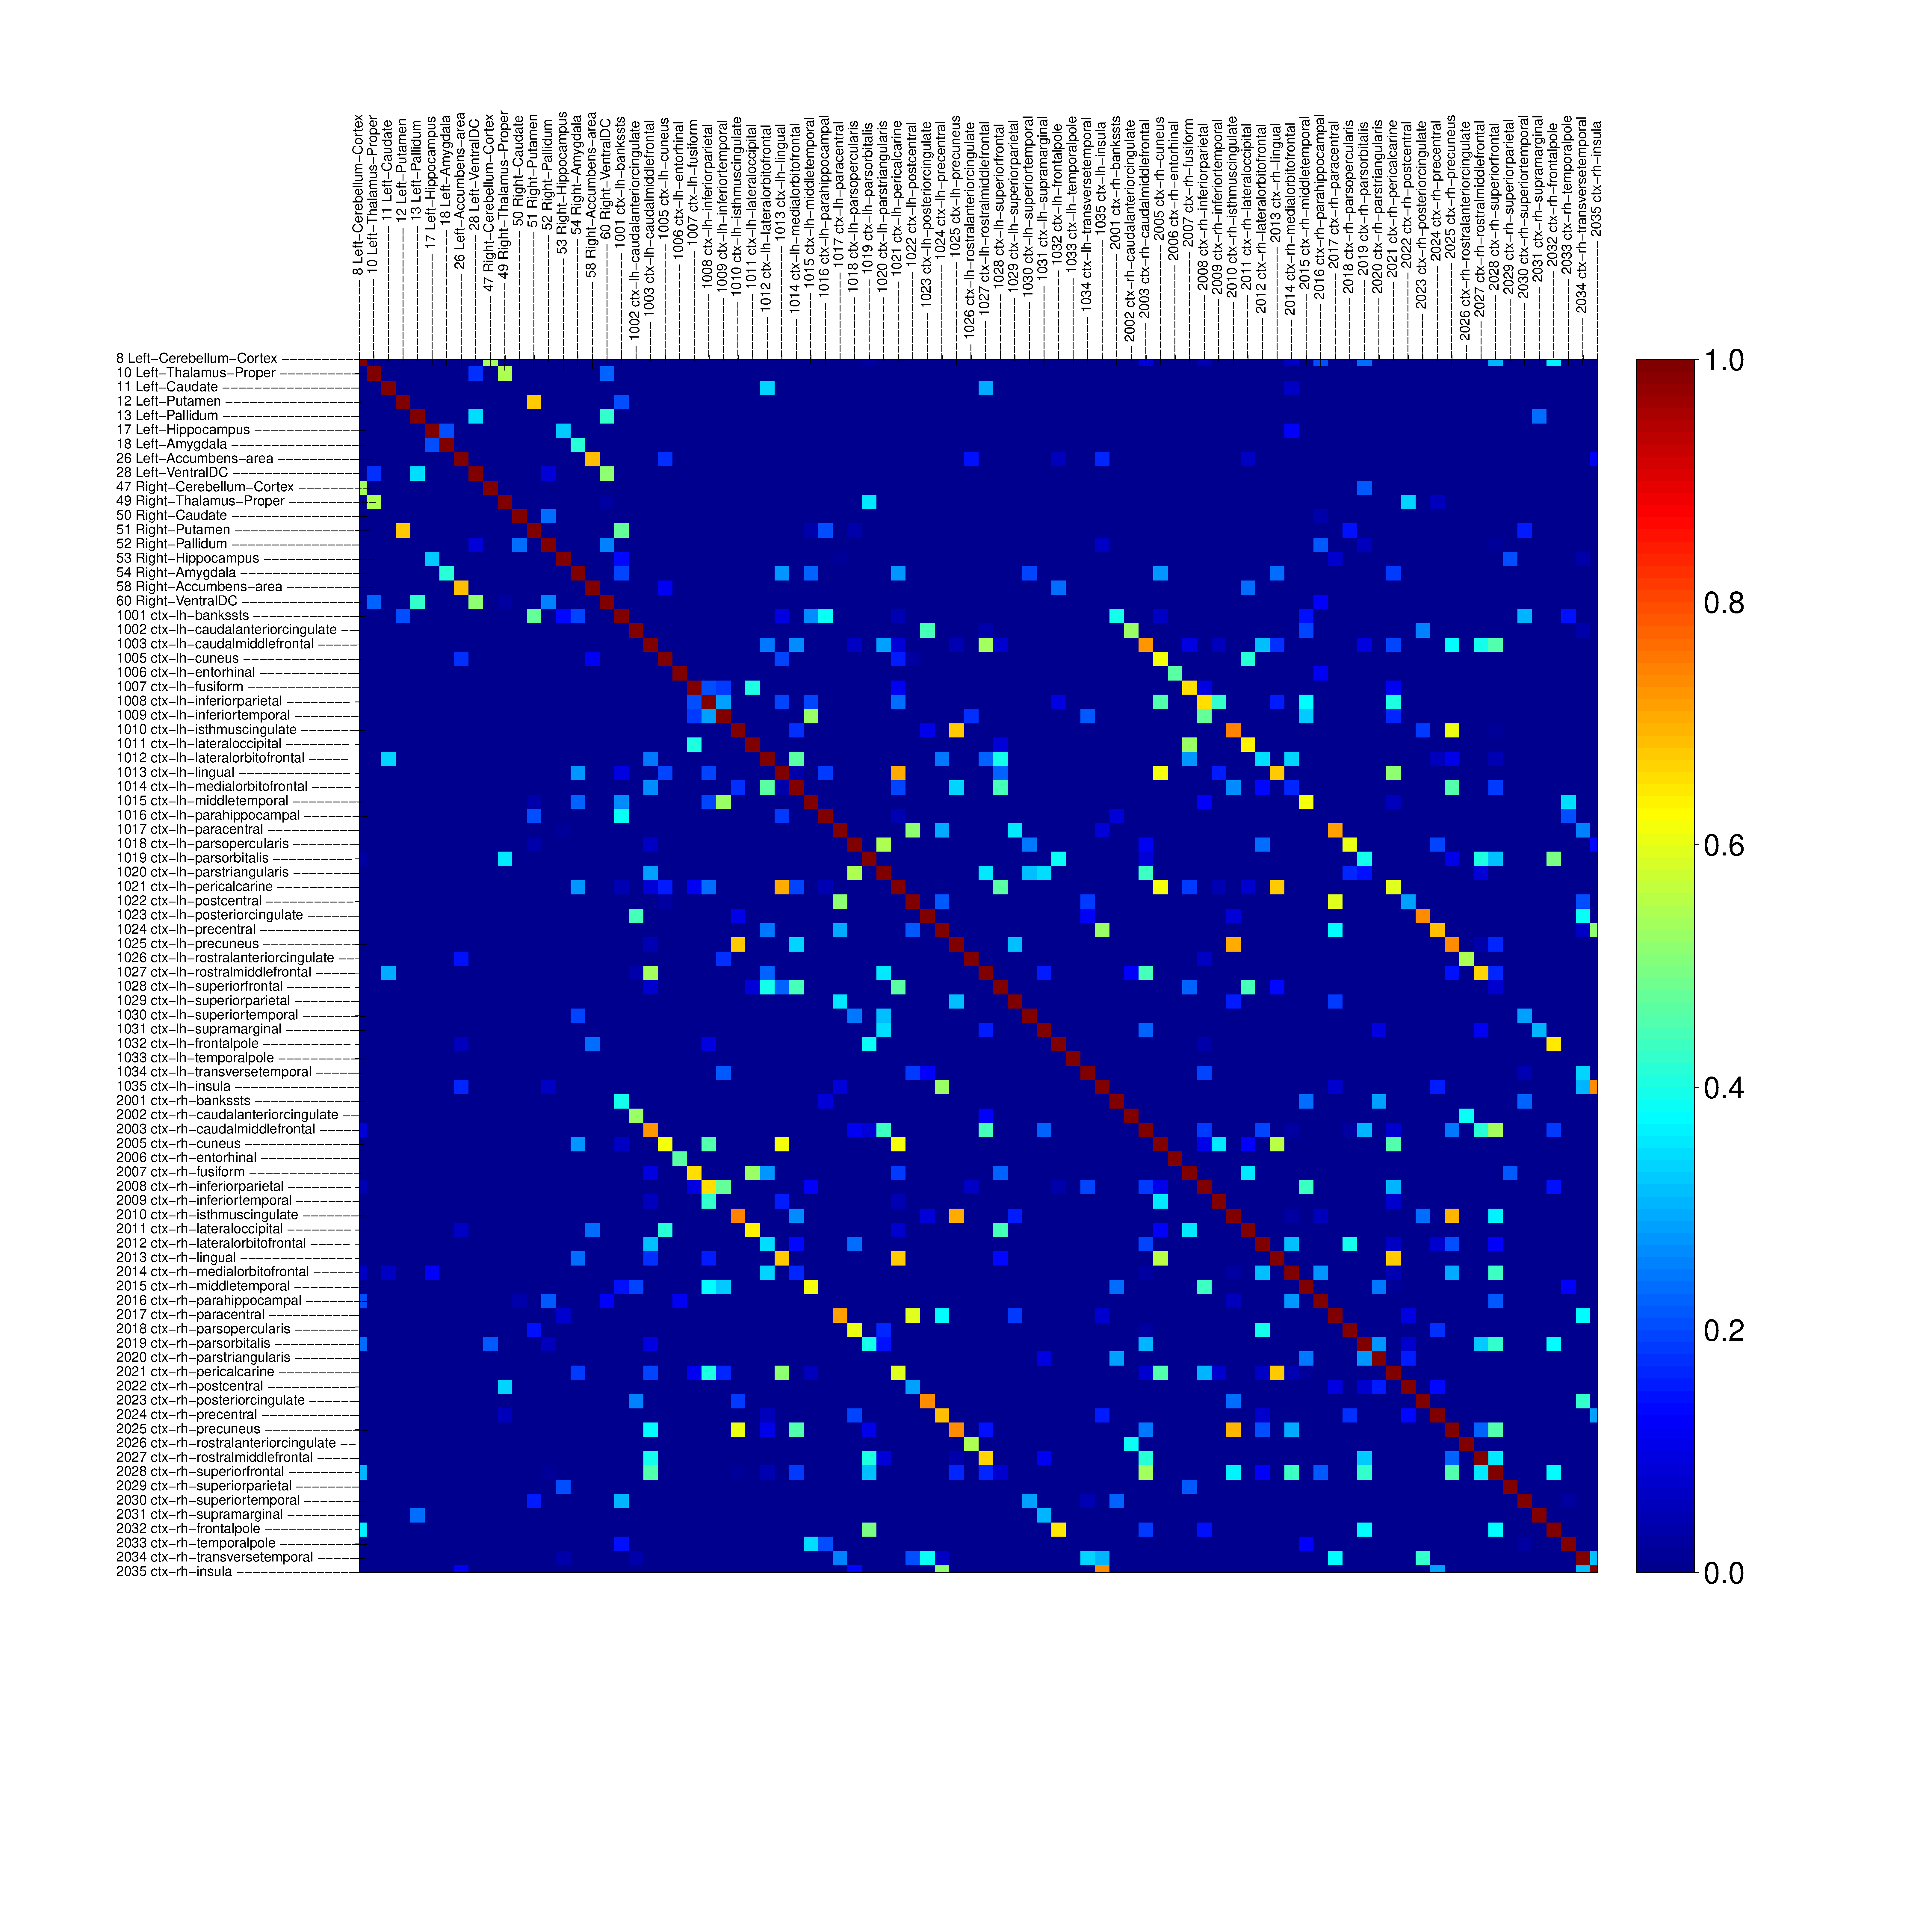
\includegraphics[width=1.1\textwidth]{img/al_hm_0.pdf}
    \caption{Heat map of absolute coherence matrix (at frequency $0$) estimated using adaptive lasso thresholding of averaged periodogram.}
    \label{fig:realdatafullalasso}
\end{figure}

\begin{figure}[p]
    \centering
    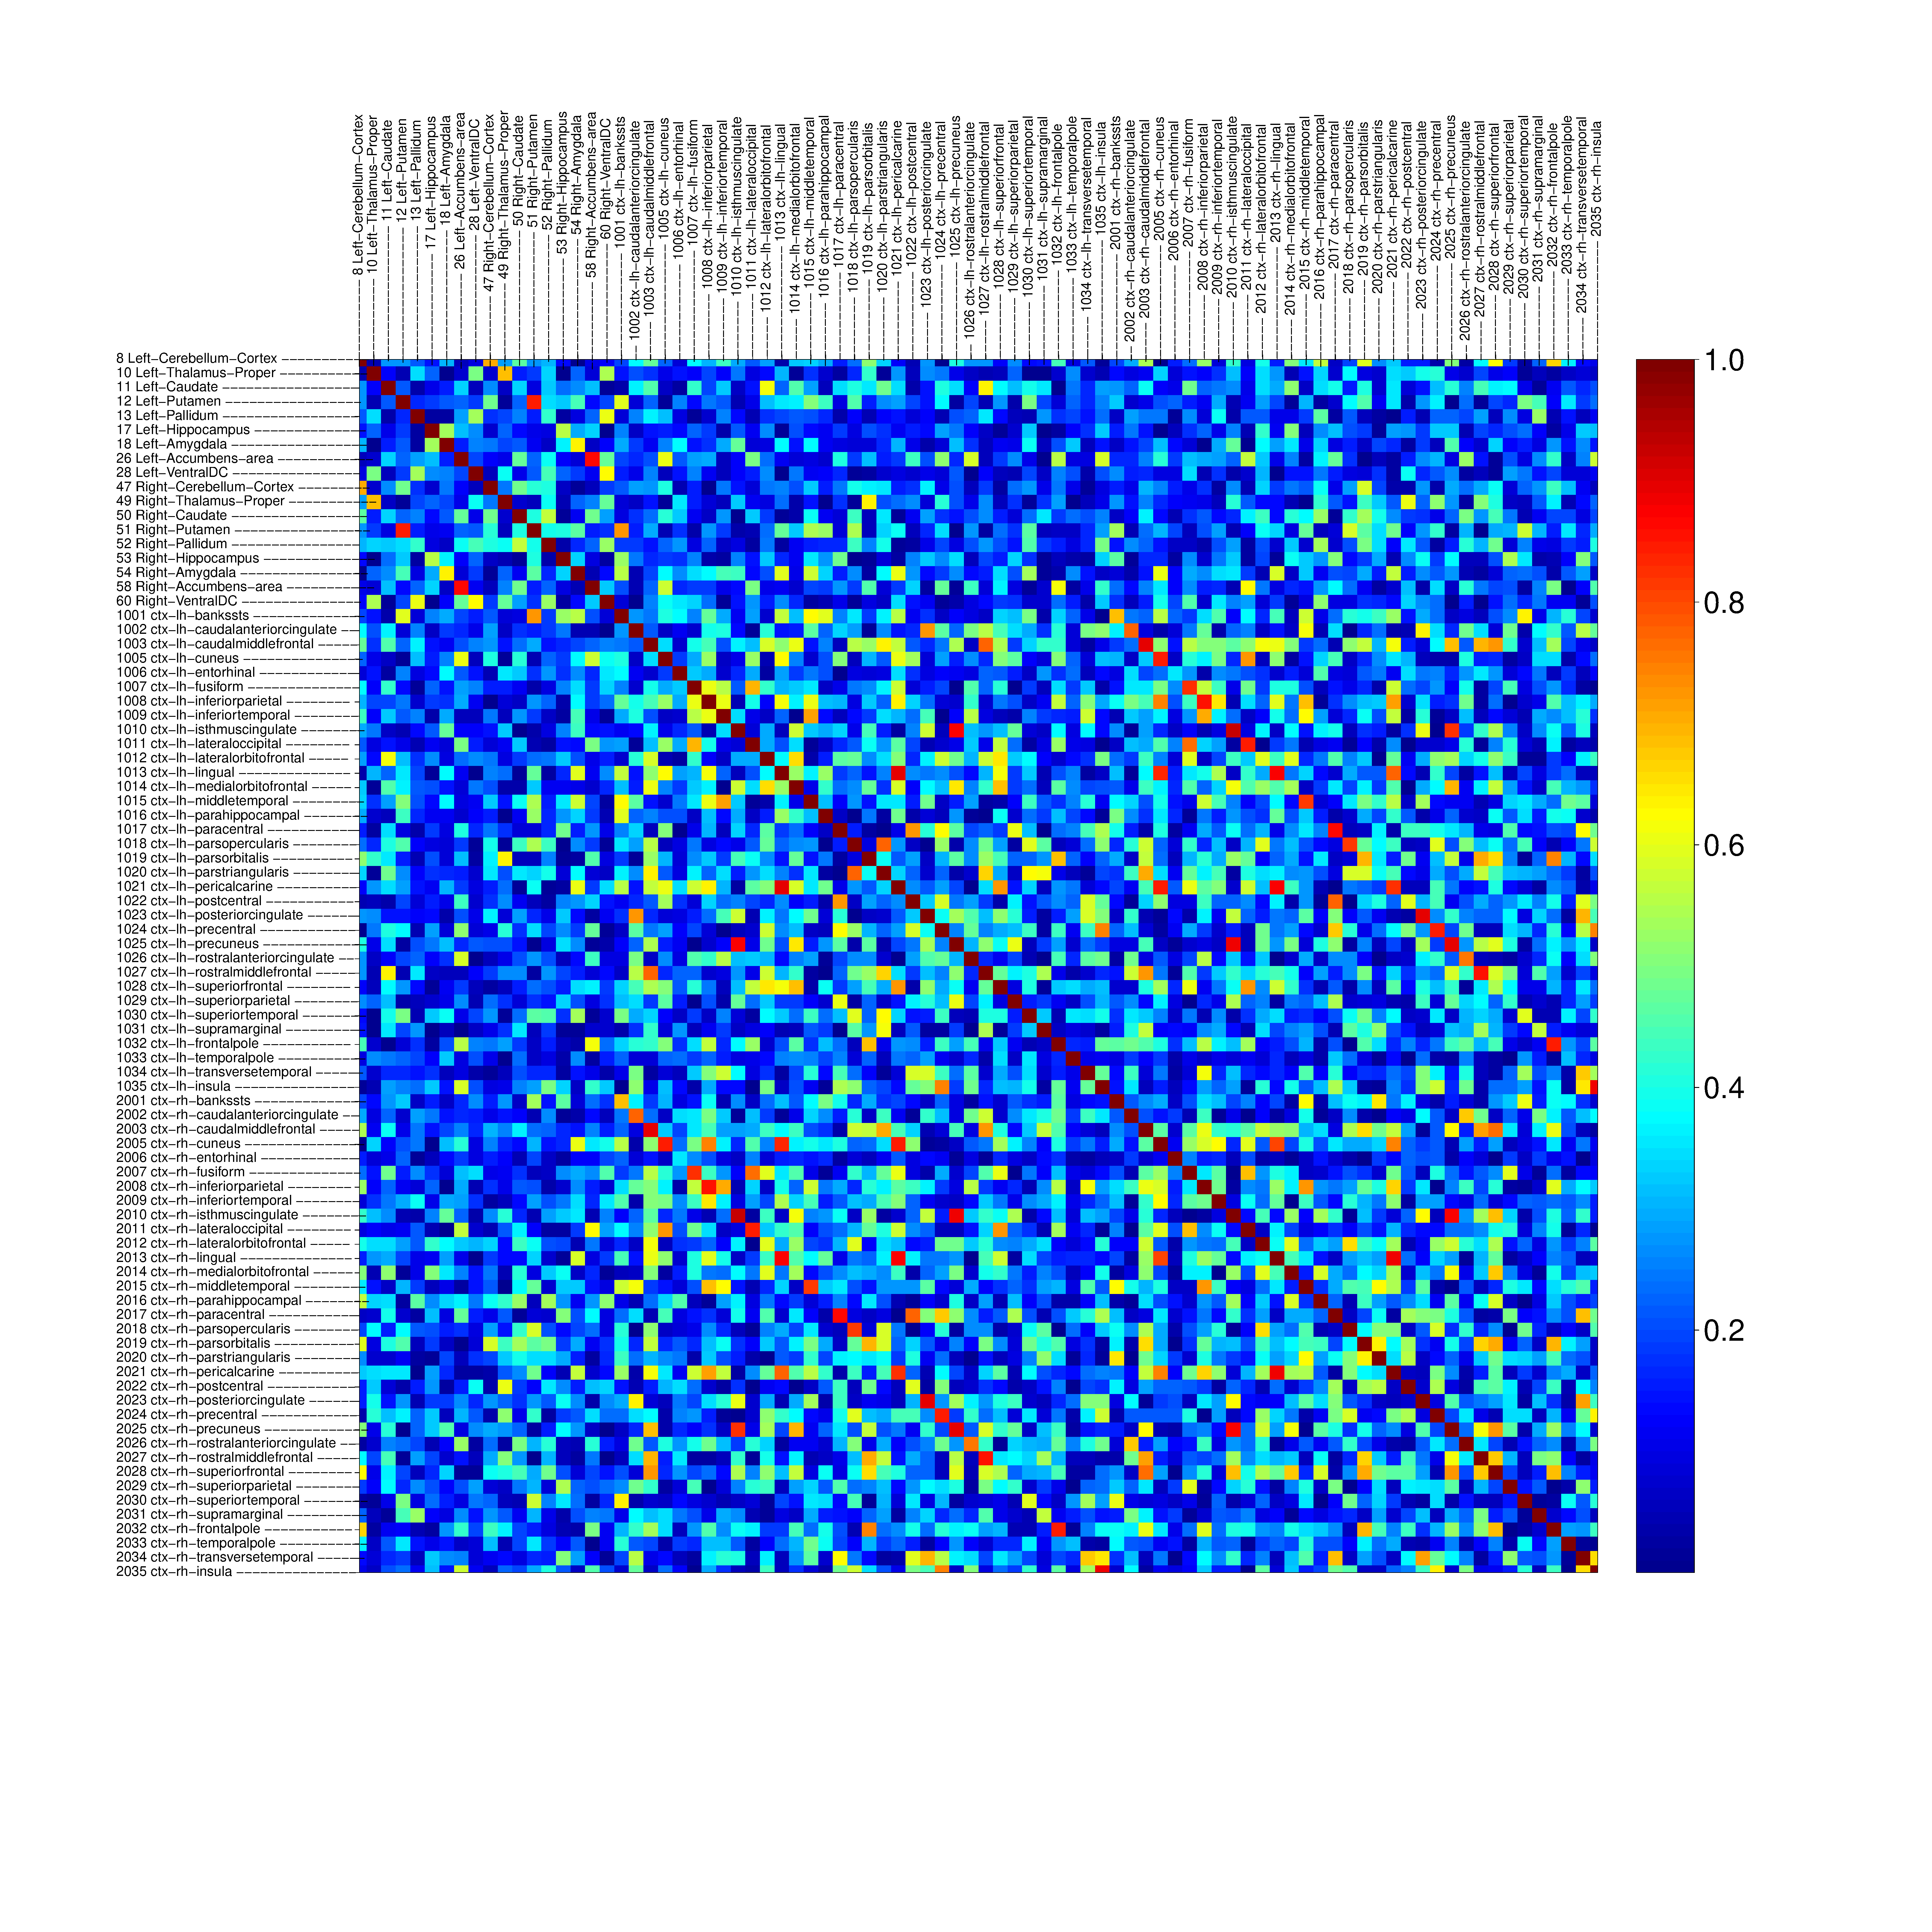
\includegraphics[width=1.1\textwidth]{img/sh_hm_0.pdf}
    \caption{Heat map of absolute coherence matrix (at frequency $0$) estimated using diagonal shrinkage of averaged periodogram.}
    \label{fig:realdatafullshrinkage}
\end{figure}



